\chapter{Scenariusze kliniczne}
W tym rozdziale zaprezentowano działanie systemu z wykorzystaniem wybranych przykładowych scenariuszy klinicznych. Wytyczne wykorzystane w tych scenariuszach zostały wcześniej skonsultowane z lekarzami, przy czym część została uproszczona na potrzeby wcześniejszych publikacji, np. \citep{SzWilk,SzWilk2}. Dla każdego scenariusza przedstawione zostały grafy reprezentujące zastosowane wytyczne. Na grafach tych zaznaczono ścieżki, które zostały wybrane podczas etapu zbierania danych pacjenta i udzielania odpowiedzi na pytania związane z węzłami decyzyjnymi. Odpowiedzi na pytania są także przedstawione w formie tekstowej. Następnie, dla każdego scenariusza przedstawiono listę możliwych konfliktów oraz zmiany, jakie należy wprowadzić w przypadku ich wystąpienia (do opisu zmian wykorzystano składnię wprowadzoną w rozdziale \ref{sect:revisions}. W celu zachowania większej zwięzłości prezentacji w opisach konfliktów i wymaganych zmian zastosowano identyfikatory węzłów -- są one przedstawione na grafach (w nawiasach po etykietach poszczególnych węzłów). Ponadto pogrubioną czcionką zaznaczono znalezione konflikty (nie wszystkie możliwe konflikty musiały wystąpić). Na końcu każdego scenariusza podane zostały grafy wynikowe. Dodane węzły w grafach wynikowych zostały oznaczone niebieską czcionką.

\section{Scenariusz 1 - atak astmy i wrzód trawienny}
Wytyczne dla ataku astmy (ang. \textit{asthma exacerbation}) przedstawiono na rys. \ref{fig:ag_ae}, natomiast wytyczne dla wrzodu trawiennego (ang. \textit{peptic ulcer}) przedstawiono na rys. \ref{fig:pu}.

\begin{figure}[H]
\centering
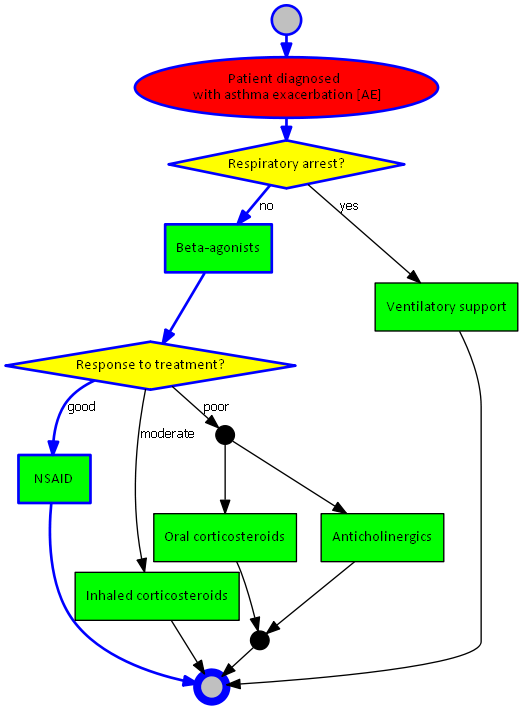
\includegraphics[scale=0.45]{img/asthma.png}
\caption{Wytyczne dla ataku astmy}
\label{fig:ag_ae}
\end{figure}

\begin{figure}[H]
\centering
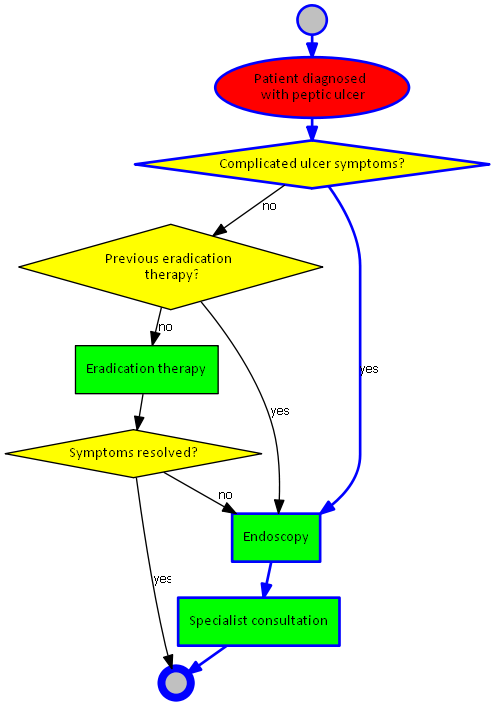
\includegraphics[scale=0.45]{img/peptic-ulcer.png}
\caption{Wytyczne dla wrzodu trawiennego}
\label{fig:pu}
\end{figure}

Dane opisujące stan pacjenta (odpowiedzi na pytania z wytycznych) są następujące:
\begin{enumerate}
\item{Atak astmy:
	\begin{itemize}
	\item{Respiratory arrest?: no (d\_arrest?no)}
	\item{Response to treatment?: good (d\_response?good)}
	\end{itemize}
}
\item{Wrzód trawienny:
	\begin{itemize}
	\item{Complicated ulcer symptoms?: yes (d\_symptoms?yes)}
	\end{itemize}
}
\end{enumerate}

Dla rozważanych wytycznych możliwe są następujące konflikty:
\begin{enumerate}
\item c\_pe a\_oral\_cortico: replace a\_oral\_cortico with a\_inh\_cortico2
\item \textbf{c\_pe a\_nsaid: add a\_ppi after a\_nsaid}
\item a\_et a\_inh\_cortico: replace a\_inh\_cortico with a\_oral\_cortico2
\end{enumerate}

% SW: W grafach wynikowych warto byłoby zaznaczyć zmodyfikowane węzły (np. innym kolorem tekstu) oraz wspomnieć o tym w opisie
Graf wynikowy dla ataku astmy przedstawiono na rys. \ref{fig:rozw_ae}, natomiast graf wynikowy dla wrzodu trawiennego jest identyczny jak ten z rys. \ref{fig:pu}.
% SW: w tym grafie należałoby zmienić opis węzła PPI -> PPI (a_ppi), aby zachować taką samą konwencję, jak w przypadku pozostałych
\begin{figure}[H]
\centering
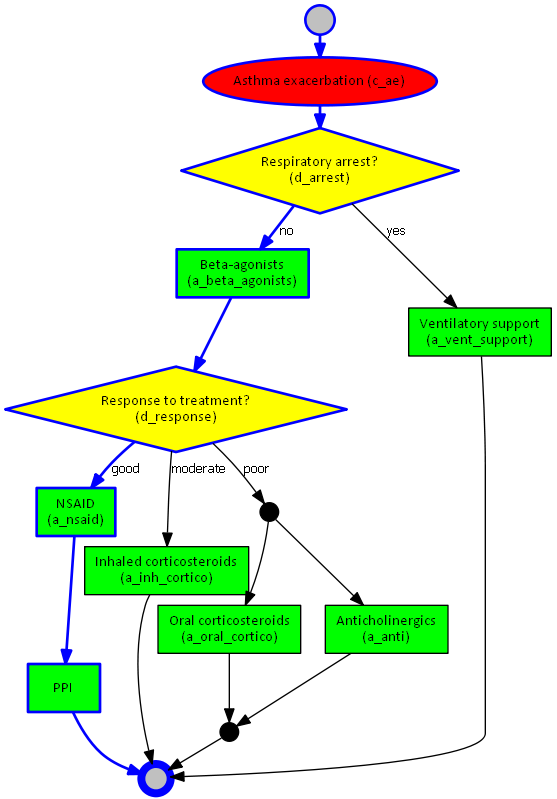
\includegraphics[scale=0.45]{img/rozwiazanie1asthma.png}
\caption{Graf wynikowy dla ataku astmy}
\label{fig:rozw_ae}
\end{figure}
\newpage
\section{Scenariusz 2 - migotanie przedsionków, przewlekła choroba nerek i nadciśnienie}
Wytyczne dla migotania przedsionków (ang. \textit{atrial fibrillation}) przedstawiono na rys. \ref{fig:afib}, dla dla przewlekłej choroby nerek (ang. \textit{chronic kidney disease}) na rys. \ref{fig:ckd}, a dla dla nadciśnienia (ang. \textit{hypertension}) na rys. \ref{fig:htn}.
% SW: tutaj zmiemiłbym identyfikator węzła decyzyjnego: d_paroxys_afib -> d_afib (większa spójność z innymi grafami). Podobna zmiana powinna zostać też wprowadzona do tekstu.

\begin{figure}[H]
\centering
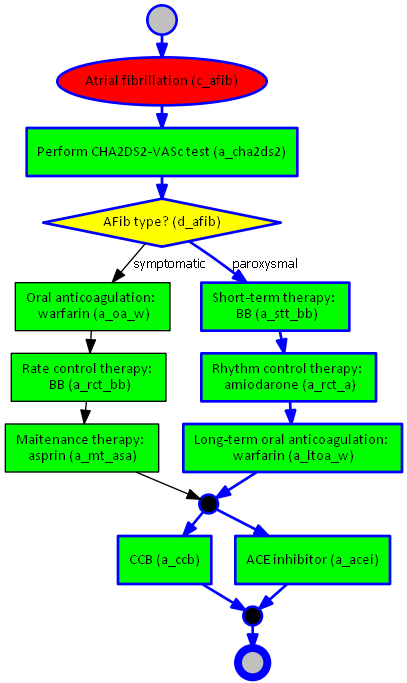
\includegraphics[scale=0.45]{img/afib-ver-4.png}
\caption{Wytyczne dla migotania przedsionków}
\label{fig:afib}
\end{figure}


\begin{figure}[H]
\centering
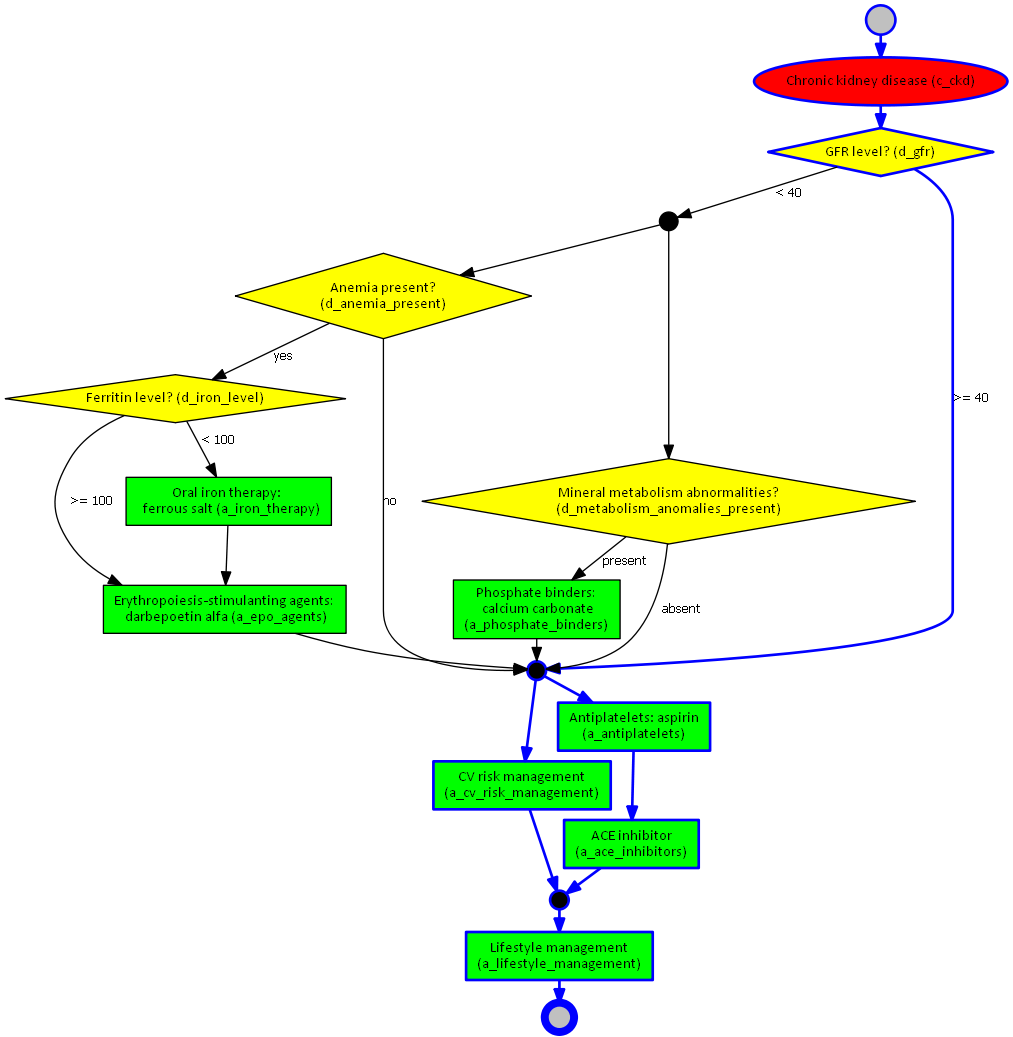
\includegraphics[scale=0.4]{img/ckd-simplified-ver-5.png}
\caption{Wytyczne dla przewlekłej choroby nerek}
\label{fig:ckd}
\end{figure}

% SW: tutaj zmieniłbym identyfikatory niektórych wierzchołków w grafie na bardziej spójne z tym, co widzieliśmy w poprzednich grafach:
% d_age_under_55 -> d_age
% d_bp_controlled_1 -> d_bp_1
% d_bp_controlled_2 -> d_bp_2
% d_bp_controlled_3 -> d_bp_3

\begin{figure}[H]
\centering
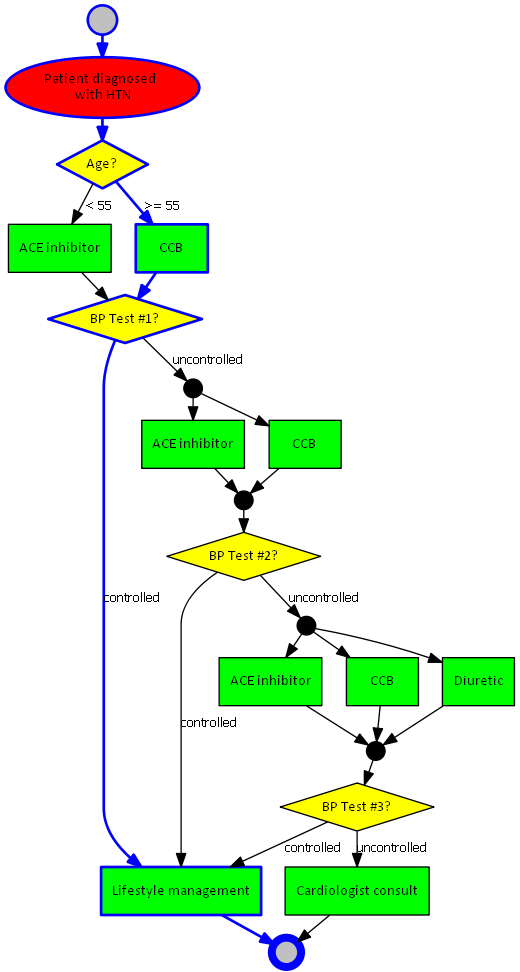
\includegraphics[scale=0.45]{img/htn-ver-3.png}
\caption{Wytyczne dla nadciśnienia}
\label{fig:htn}
\end{figure}

Dane opisujące stan pacjenta (odpowiedzi na pytania z wytycznych) są następujące:
\begin{enumerate}
\item{Migotanie przedsionków:
	\begin{itemize}
	\item{AFib type?: paroxysmal (d\_afib?paroxysmal)}
	\end{itemize}
}
\item{Przewlekła choroba nerek:
	\begin{itemize}
	\item{GFR level?: >=40 (d\_gfr?>=40)}
	\end{itemize}
}
\item{Nadciśnienie:
	\begin{itemize}
	\item{Age?: >=55 (d\_age?>=55)}
	\item{BP Test \#1?: controlled (d\_bp\_1?controlled)}
	\end{itemize}
}
\item Dodatkowe dane, które nie pojawiły się jawnie w wytycznych i które zostały uzupełnione podczas fazy poszukiwania konfliktów:
	\begin{itemize}
	\item{CHA2DS2-VASc = 5 (\&CHA2DS2-VASc?5)}
	\end{itemize}
\end{enumerate}

Dla rozważanych wytycznych możliwe są następujące konflikty:
\begin{enumerate}
\item \textbf{c\_htn c\_ckd: remove a\_step1\_acei, remove a\_step1\_ccb}
\item \textbf{c\_afib c\_ckd c\_htn: remove a\_step3\_diuretric}
\item \textbf{c\_afib c\_ckd: replace a\_antiplatelets with a\_warfarin, replace a\_rct\_a with a\_bb}
\item \textbf{c\_afib c\_ckd \&CHA2DS2-VASc>2: replace a\_mt\_asa with a\_warfarin\_2}
\item c\_afib c\_ckd \&CHA2DS2-VASc<=1: replace a\_oa\_w with a\_aspirin\_1, replace a\_ltoa\_w with a\_aspirin\_2
\end{enumerate}

Graf wynikowy dla migotania przedsionków przedstawiono na rys. \ref{fig:rozw_afib}, dla przewlekłej choroby nerek na rys. \ref{fig:rozw_ckd}, natomiast dla nadciśnienia na rys. \ref{fig:rozw_htn}.

% SW: W tym grafie powinien zmienić Pan opis węzła BB -> BB (a_bb)
\begin{figure}[H]
\centering
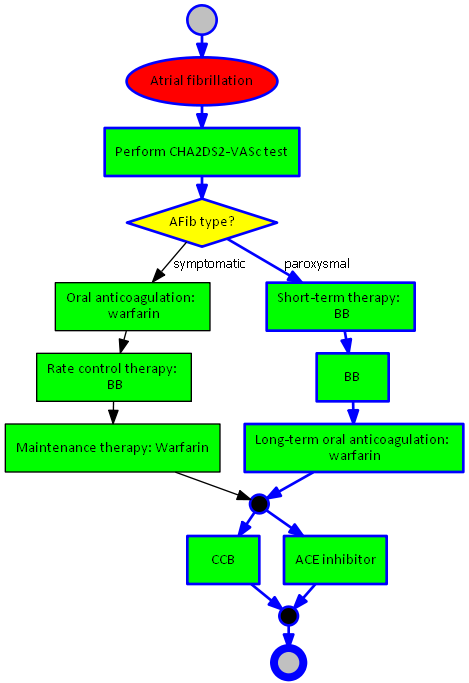
\includegraphics[scale=0.45]{img/rozwiazanie1afib-ver-4.png}
\caption{Graf wynikowy dla migotania przedsionków}
\label{fig:rozw_afib}
\end{figure}

% SW: w tym grafie zmieniamy Warfarin -> Warfarin (a_warfarin) oraz Maintenance therapy: warfarin -> Maintenance therapy: warfarin (a_warfarin_2)
\begin{figure}[H]
\centering
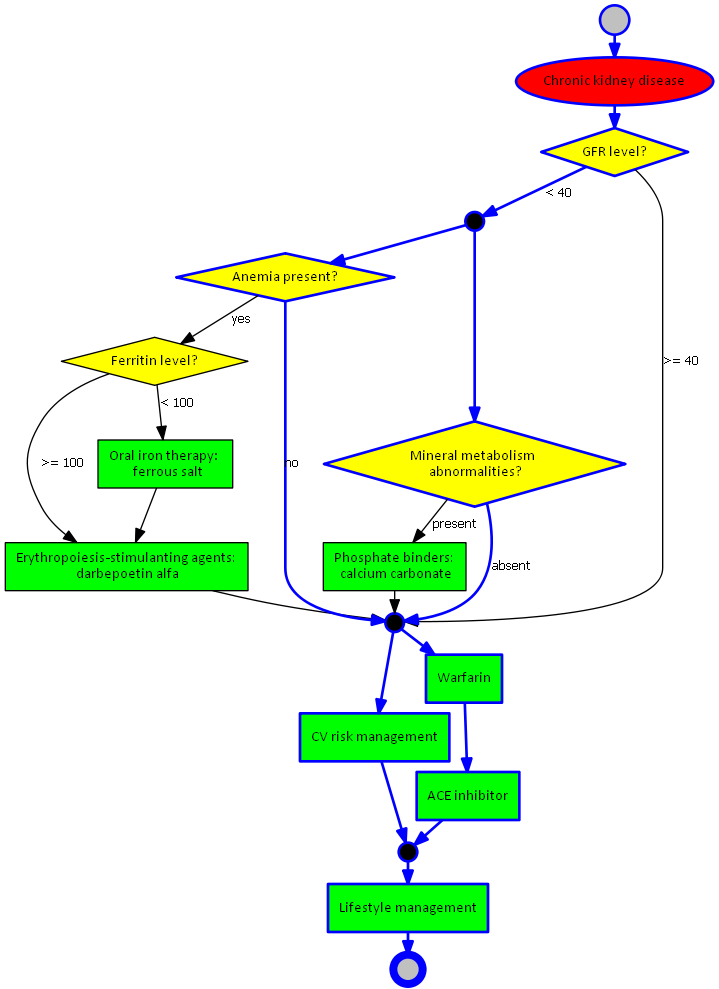
\includegraphics[scale=0.4]{img/rozwiazanie1ckd-simplified-ver-5.png}
\caption{Graf wynikowy dla przewlekłej choroby nerek}
\label{fig:rozw_ckd}
\end{figure}
\begin{figure}[H]
\centering
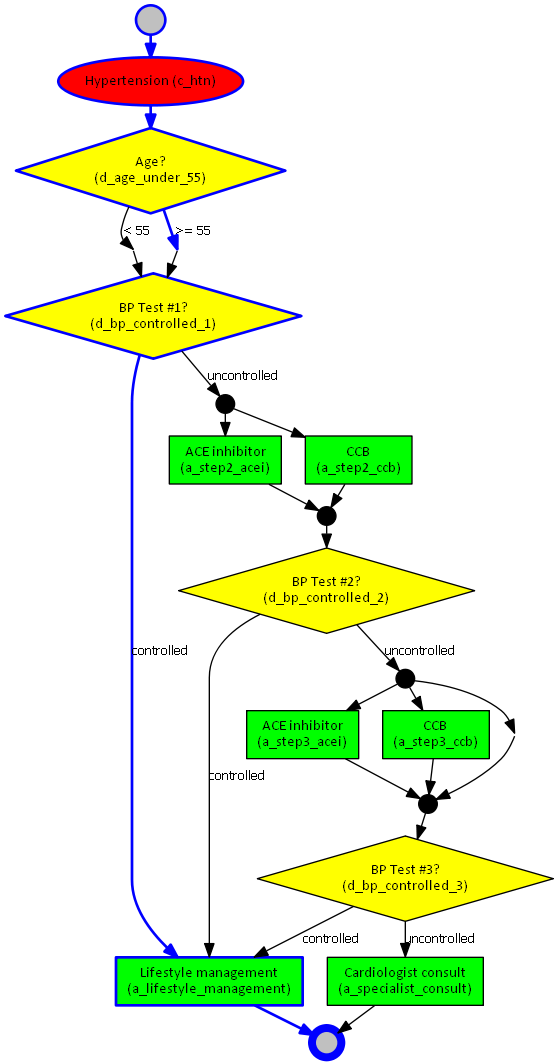
\includegraphics[scale=0.45]{img/rozwiazanie1htn-ver-3.png}
\caption{Graf wynikowy dla nadciśnienia}
\label{fig:rozw_htn}
\end{figure}


\newpage
\section{Scenariusz 3 - wrzód dwunastnicy i przemijający atak niedokrwienny}
Wytyczne dla wrzodu dwunastnicy (ang. \textit{duodenal ulcer}) przedstawiono na rys. \ref{fig:du}, natomiast dla przemijającego ataku niedokrwiennego (ang. \textit{transient ischemic attack}) na rys. \ref{fig:tia}.
\begin{figure}[H]
\centering
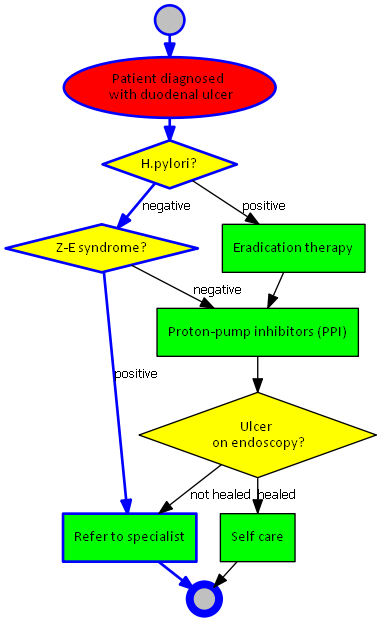
\includegraphics[scale=0.45]{img/du.png}
\caption{Wytyczne dla wrzodu dwunastnicy}
\label{fig:du}
\end{figure}


\begin{figure}[H]
\centering
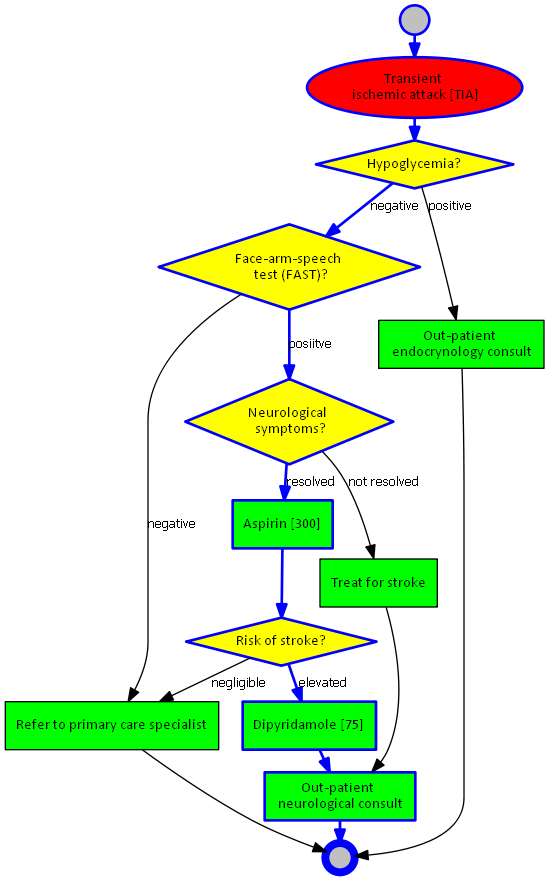
\includegraphics[scale=0.45]{img/tia.png}
\caption{Wytyczne dla przemijającego ataku niedokrwiennego}
\label{fig:tia}
\end{figure}

Dane opisujące stan pacjenta (odpowiedzi na pytania z wytycznych) są następujące:
\begin{enumerate}
\item{Wrzód dwunastnicy:
	\begin{itemize}
	\item{H.pylori?: negative (d\_hyplori?negative)}
	\item{Z-E syndrome?: positive (d\_ze\_syndrome?positive)}
	\end{itemize}
}
\item{Przemijający atak niedokrwienny:
	\begin{itemize}
	\item{Hypoglycemia?: negative (d\_hypoglycemia?negative)}
	\item{Face-arm-speech test (FAST)?: positive (d\_fast?positive)}
	\item{Neurological symptoms?: resolved (d\_neuro\_symptoms?resolved)}
	\item{Risk of stroke?: elevated (d\_stroke\_risk?elevated)}
	\end{itemize}
}
\end{enumerate}
Dla rozważanych wytycznych możliwe są następujące konflikty:
\begin{enumerate}
\item c\_du a\_aspirin not(a\_ppi) not(a\_dipyridamole): replace a\_aspirin with a\_cl
\item \textbf{c\_du a\_aspirin not(a\_ppi) a\_dipyridamole: add a\_ppi\_2 after d\_ze\_synd\-rome?positive, decrease\_dosage a\_aspirin 50}
\end{enumerate}

Graf wynikowy dla wrzodu dwunastnicy przedstawiono na rys. \ref{fig:rozw_du}, natomiast dla przemijającego ataku niedokrwiennego na rys. \ref{fig:rozw_tia}.

% SW: W tym grafie proszę zmienić Proton-pump inhibitors (PPI) -> Proton-pump inhibitors (a_ppi_2)
\begin{figure}[H]
\centering
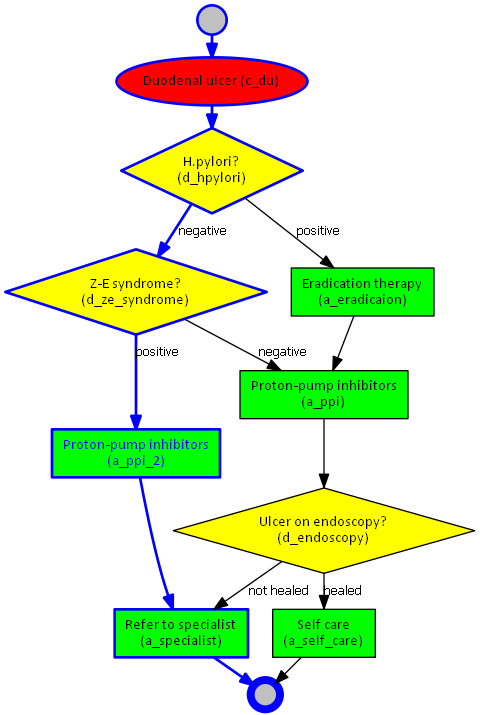
\includegraphics[scale=0.5]{img/rozwiazanie1du.png}
\caption{Graf wynikowy dla wrzodu dwunastnicy}
\label{fig:rozw_du}
\end{figure}
\begin{figure}[H]
\centering
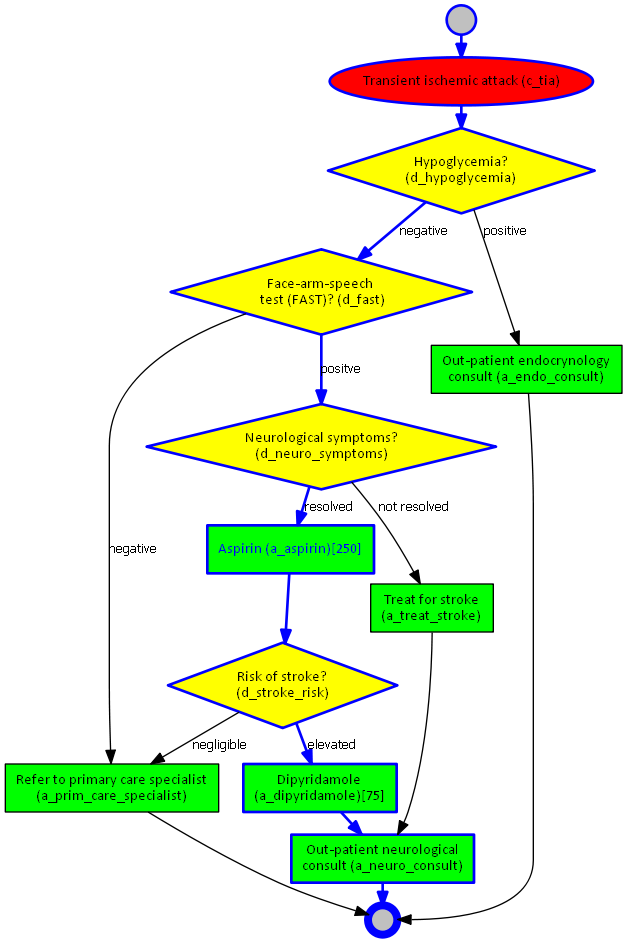
\includegraphics[scale=0.5]{img/rozwiazanie1tia.png}
\caption{Graf wynikowy dla przemijającego ataku niedokrwiennego}
\label{fig:rozw_tia}
\end{figure}
